% !TEX program = pdflatex
% Interim seminar presentation for the SEMINAR item-reviser benchmark.
% Build from this folder with: pdflatex item_reviser_interim_presentation.tex

\documentclass[aspectratio=169,10pt]{beamer}

\usetheme{Madrid}
\usecolortheme{default}

\usepackage[utf8]{inputenc}
\usepackage[T1]{fontenc}
\usepackage{graphicx}
\usepackage{booktabs}
\usepackage{array}
\usepackage{tabularx}
\usepackage{multirow}
\usepackage{xcolor}
\usepackage{colortbl}
\usepackage{ragged2e}
\usepackage{tikz}

% ---------- Theme colors ----------
\definecolor{SeminarNavy}{HTML}{06194A}
\definecolor{SeminarBlue}{HTML}{123A7A}
\definecolor{SeminarLightBlue}{HTML}{EAF1FF}
\definecolor{SeminarGreen}{HTML}{136F45}
\definecolor{SeminarOrange}{HTML}{B45F06}
\definecolor{SeminarRed}{HTML}{9F1D20}
\definecolor{SeminarGray}{HTML}{F2F3F5}
\definecolor{SeminarDarkGray}{HTML}{444444}

\setbeamercolor{title}{fg=SeminarNavy}
\setbeamercolor{frametitle}{fg=SeminarNavy,bg=white}
\setbeamercolor{structure}{fg=SeminarNavy}
\setbeamercolor{block title}{fg=white,bg=SeminarNavy}
\setbeamercolor{block body}{fg=black,bg=SeminarLightBlue}
\setbeamercolor{alerted text}{fg=SeminarRed}
\setbeamerfont{title}{series=\bfseries,size=\Large}
\setbeamerfont{frametitle}{series=\bfseries,size=\large}
\setbeamertemplate{navigation symbols}{}
\setbeamertemplate{footline}[frame number]

% ---------- Convenience commands ----------
\newcommand{\good}[1]{\textcolor{SeminarGreen}{\textbf{#1}}}
\newcommand{\bad}[1]{\textcolor{SeminarRed}{\textbf{#1}}}
\newcommand{\warn}[1]{\textcolor{SeminarOrange}{\textbf{#1}}}
\newcommand{\cat}[1]{\texttt{\detokenize{#1}}}
\newcommand{\tight}{\setlength{\itemsep}{2pt}\setlength{\parskip}{0pt}}
\newcommand{\source}[1]{\vspace{2mm}{\tiny\textcolor{SeminarDarkGray}{#1}}}

\title[Item-Reviser Interim Results]{Interim Results: LLM Item-Reviser Benchmark}
\subtitle{18-experiment MLflow evaluation on the final 200-item gold set}
\author{Seminar presentation draft}
\date{July 2026}

\begin{document}

% ============================================================
\begin{frame}[plain]
\centering
\vspace{1.1cm}
{\color{SeminarNavy}\Huge\bfseries Interim Results: LLM Item-Reviser Benchmark\par}
\vspace{0.35cm}
{\Large 18-experiment MLflow evaluation on the final 200-item gold set\par}
\vspace{0.55cm}
{\color{SeminarNavy}\rule{0.82\linewidth}{1.2pt}\par}
\vspace{0.65cm}
{\large Seminar presentation draft\par}
\vspace{0.3cm}
{\normalsize Survey item quality checking and revision\par}
\vspace{0.55cm}
{\normalsize July 2026\par}
\end{frame}

% ============================================================
\begin{frame}{Purpose of this interim presentation}
\begin{block}{Goal}
Evaluate whether a zero-shot LLM system can \textbf{detect} questionnaire-design flaws and \textbf{revise} flawed survey items while avoiding unnecessary changes to clean controls.
\end{block}

\vspace{2mm}
\begin{columns}[T,onlytextwidth]
\begin{column}{0.49\textwidth}
\textbf{Experiment matrix}
\begin{itemize}\tight
  \item 3 models: Mistral 7B, Gemma 2 9B, Qwen 3.5 9B
  \item 2 pipelines: baseline vs. orchestrated
  \item 3 modes: detection-only, oracle-revision, end-to-end
  \item Total: \textbf{18 runs} over the same 200-item dataset
\end{itemize}
\end{column}
\begin{column}{0.49\textwidth}
\textbf{Interim focus}
\begin{itemize}\tight
  \item Main metric block: taxonomy-label detection
  \item Main system comparison: Qwen baseline vs. Qwen orchestrated
  \item Error analysis: under-performing categories and why
  \item Design implication: LLM-only router vs. hybrid checks
\end{itemize}
\end{column}
\end{columns}
\end{frame}

% ============================================================
% ============================================================
\begin{frame}{Benchmark dataset: final 200-item gold set}
\begin{columns}[T,onlytextwidth]
\begin{column}{0.48\textwidth}
\begin{block}{Dataset composition}
\centering
\small
\begin{tabular}{lr}
\toprule
Property & Count\\
\midrule
Total survey items & \textbf{200}\\
Clean controls & \textbf{40}\\
Flawed items & \textbf{160}\\
Single-label flawed items & \textbf{128}\\
Multi-label flawed items & \textbf{32}\\
Taxonomy labels & \textbf{16}\\
Appearances per label & \textbf{12}\\
\bottomrule
\end{tabular}
\end{block}
\end{column}

\begin{column}{0.48\textwidth}
\begin{block}{Why this matters}
\begin{itemize}\tight
  \item Clean controls test false positives and overcorrection.
  \item Single-label items isolate category-specific detection.
  \item Multi-label items test realistic compound flaws.
  \item Balanced label counts make category-level comparisons easier.
\end{itemize}
\end{block}

\vspace{2mm}
\begin{alertblock}{Interim status}
This is a structurally validated gold-candidate dataset, but final human/professor signoff is still recommended before calling it externally validated.
\end{alertblock}
\end{column}
\end{columns}
\end{frame}
% ============================================================
% ============================================================
\begin{frame}{Benchmark taxonomy: balanced across 16 flaw labels}
\scriptsize
\centering
\begin{tabular}{lrr@{\hspace{8mm}}lrr}
\toprule
Label & Total & Single & Label & Total & Single\\
\midrule
\cat{leading_question} & 12 & 8 &
\cat{loaded_question} & 12 & 8\\
\cat{double_barreled} & 12 & 8 &
\cat{recall_error} & 12 & 8\\
\cat{vague_ambiguous} & 12 & 8 &
\cat{sensitive_topic_direct} & 12 & 8\\
\cat{social_desirability} & 12 & 8 &
\cat{negative_wording} & 12 & 8\\
\cat{open_closed_mismatch} & 12 & 8 &
\cat{agree_disagree_scale} & 12 & 8\\
\cat{unbalanced_scale} & 12 & 8 &
\cat{incomplete_options} & 12 & 8\\
\cat{non_exclusive_options} & 12 & 8 &
\cat{missing_scale_labels} & 12 & 8\\
\cat{too_many_scale_points} & 12 & 8 &
\cat{polarity_mismatch} & 12 & 8\\
\bottomrule
\end{tabular}

\vspace{4mm}
\begin{block}{Design implication}
Each label appears exactly \textbf{12 times}: \textbf{8} as a single-label flaw and \textbf{4} inside multi-label items. This supports both isolated category analysis and more realistic compound-error evaluation.
\end{block}
\end{frame}

% ============================================================
\begin{frame}{Topic distribution: broad coverage across survey domains}
\scriptsize
\centering
\begin{tabular}{lrlr}
\toprule
Topic & Count & Topic & Count\\
\midrule
\cat{education} & 19 &
\cat{health} & 19\\
\cat{public services} & 19 &
\cat{university life} & 16\\
\cat{family/household} & 16 &
\cat{technology} & 15\\
\cat{environment} & 15 &
\cat{politics/public policy} & 13\\
\cat{mobility} & 13 &
\cat{work} & 13\\
\cat{media/culture} & 13 &
\cat{finances} & 12\\
\cat{labor} & 10 &
\cat{sensitive behaviors} & 7\\
\bottomrule
\end{tabular}

\vspace{4mm}
\begin{block}{Why topic diversity matters}
The benchmark is not limited to one questionnaire domain. It tests whether the item-reviser can generalize across public policy, education, health, technology, work, household, mobility, media, and sensitive-behavior contexts.
\end{block}
\end{frame}
% ============================================================
\begin{frame}{Two evaluation modes answer different questions}
\begin{columns}[T,onlytextwidth]
\begin{column}{0.32\textwidth}
\begin{block}{Detection-only}
Can the model identify known taxonomy labels?
\vspace{1mm}

\textbf{No revision quality claim.}
\end{block}
\end{column}
\begin{column}{0.32\textwidth}
\begin{block}{Oracle-revision}
Can the model revise when the gold flaw category is supplied?
\vspace{1mm}

\textbf{Isolates revision ability.}
\end{block}
\end{column}
\begin{column}{0.32\textwidth}
\begin{block}{End-to-end}
Can the full system detect and revise without gold help?
\vspace{1mm}

\textbf{Most realistic system test.}
\end{block}
\end{column}
\end{columns}

\vspace{4mm}
\begin{alertblock}{Interpretation rule}
Oracle-revision results should not be interpreted as detection performance. They answer a different question: revision quality under known-error conditions.
\end{alertblock}
\end{frame}

% ============================================================
\begin{frame}{Baseline workflow}
\centering
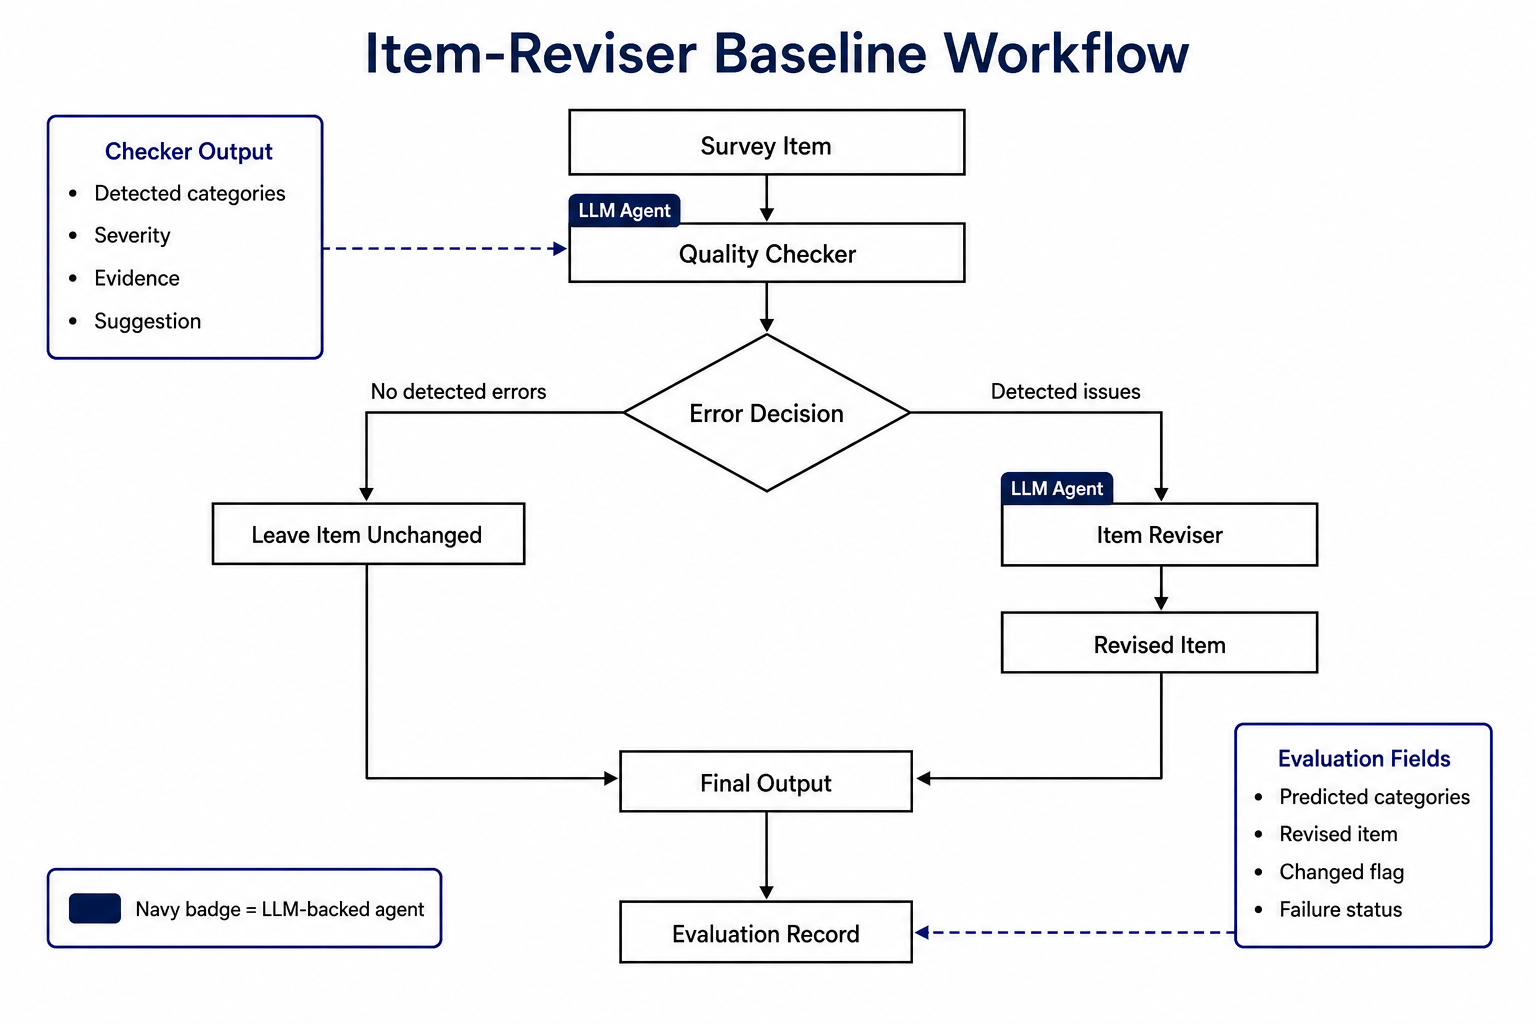
\includegraphics[width=0.88\textwidth,height=0.78\textheight,keepaspectratio]{item_reviser_baseline_agents_academic.png}
\end{frame}

% ============================================================
\begin{frame}{Orchestration workflow}
\centering

\includegraphics[width=0.92\textwidth,height=0.82\textheight,keepaspectratio]{item_reviser_orchestration_agents_academic.png}
\end{frame}

% ============================================================
\begin{frame}{Metric definitions used in the analysis}
\small
\begin{tabularx}{\textwidth}{>{\bfseries}p{0.28\textwidth}X}
\toprule
Metric & Meaning\\
\midrule
Precision / recall / F1 & Taxonomy-label detection quality against known error labels.\\
Exact match & Exact match of the predicted taxonomy-label set, not exact rewrite matching.\\
Clean false-positive rate & Fraction of clean controls where the model predicted at least one error label.\\
Overcorrection rate & Fraction of clean controls where the output item was changed.\\
Exact revision rate & Fraction of items whose rewritten question and options exactly match the expected revision.\\
Failure rate & Fraction of items where parsing, schema, or pipeline failure was recorded.\\
\bottomrule
\end{tabularx}

\vspace{3mm}
\begin{alertblock}{Revision metric caveat}
Exact revision rate is a harsh proxy. A valid rewrite can differ from the reference rewrite. Use it for diagnostics, not as the sole revision-quality measure.
\end{alertblock}
\end{frame}

% ============================================================
\section{Results}

\begin{frame}{End-to-end results: all systems}
\scriptsize
\resizebox{\textwidth}{!}{%
\begin{tabular}{llrrrrrrr}
\toprule
Model & Pipeline & F1 & Precision & Recall & Exact match & Clean FPR & Overcorr. & Failed\\
\midrule
Mistral 7B v0.3 & baseline & 0.170 & 0.137 & 0.224 & 0.070 & 1.000 & 1.000 & 0\\
Mistral 7B v0.3 & orchestrated & 0.117 & 0.132 & 0.104 & 0.145 & 0.625 & 0.625 & 0\\
Gemma 2 9B & baseline & 0.387 & 0.366 & 0.411 & 0.270 & 1.000 & 1.000 & 0\\
Gemma 2 9B & orchestrated & 0.333 & 0.357 & 0.313 & 0.280 & 0.725 & 0.725 & 0\\
\rowcolor{SeminarLightBlue}
Qwen 3.5 9B & baseline & \good{0.503} & 0.390 & \good{0.708} & 0.250 & 0.250 & 0.225 & 2\\
\rowcolor{SeminarLightBlue}
Qwen 3.5 9B & orchestrated & 0.492 & \good{0.490} & 0.495 & \good{0.315} & \good{0.100} & \good{0.075} & \good{0}\\
\bottomrule
\end{tabular}}

\vspace{3mm}
\begin{block}{Interpretation}
Baseline Qwen is the strongest high-recall detector. Orchestrated Qwen is slightly lower on F1, but substantially better at avoiding false positives and unnecessary changes on clean controls.
\end{block}
\end{frame}

% ============================================================
\begin{frame}{End-to-end metric trade-off: why Qwen orchestrated matters}
\begin{columns}[T,onlytextwidth]
\begin{column}{0.46\textwidth}
\begin{block}{Qwen baseline}
\begin{itemize}\tight
  \item Highest F1: \good{0.503}
  \item Highest recall: \good{0.708}
  \item Useful when missing errors is costly
  \item But it changes 22.5\% of clean controls and has 2 parse failures
\end{itemize}
\end{block}
\end{column}
\begin{column}{0.46\textwidth}
\begin{block}{Qwen orchestrated}
\begin{itemize}\tight
  \item Higher precision: \good{0.490}
  \item Better exact label-set match: \good{0.315}
  \item Lower clean false-positive rate: \good{0.100}
  \item Lower overcorrection: \good{0.075}
  \item No parse failures
\end{itemize}
\end{block}
\end{column}
\end{columns}

\vspace{4mm}
\begin{alertblock}{Practical conclusion}
Use \textbf{Qwen baseline} as the high-recall detector comparison, but present \textbf{Qwen orchestrated} as the strongest practical end-to-end item-revision system.
\end{alertblock}
\end{frame}

% ============================================================
\begin{frame}{Detection-only results confirm the same pattern}
\scriptsize
\resizebox{\textwidth}{!}{%
\begin{tabular}{llrrrrr}
\toprule
Model & Pipeline & F1 & Precision & Recall & Exact match & Clean FPR\\
\midrule
Mistral 7B v0.3 & baseline & 0.170 & 0.137 & 0.224 & 0.070 & 1.000\\
Mistral 7B v0.3 & orchestrated & 0.117 & 0.132 & 0.104 & 0.145 & 0.625\\
Gemma 2 9B & baseline & 0.387 & 0.366 & 0.411 & 0.270 & 1.000\\
Gemma 2 9B & orchestrated & 0.333 & 0.357 & 0.313 & 0.280 & 0.725\\
\rowcolor{SeminarLightBlue}
Qwen 3.5 9B & baseline & \good{0.505} & 0.390 & \good{0.719} & 0.250 & 0.250\\
\rowcolor{SeminarLightBlue}
Qwen 3.5 9B & orchestrated & 0.492 & \good{0.490} & 0.495 & \good{0.315} & \good{0.100}\\
\bottomrule
\end{tabular}}

\vspace{3mm}
\begin{block}{Takeaway}
Detection-only and end-to-end detection metrics are nearly identical. The revision stage does not change the main detection story; it mainly affects output robustness and overcorrection.
\end{block}
\end{frame}

% ============================================================
\begin{frame}{Automatic revision-quality proxies}
\scriptsize
\resizebox{\textwidth}{!}{%
\begin{tabular}{llrrrr}
\toprule
Model & Pipeline & Exact revision & Question similarity & Option Jaccard & Changed rate\\
\midrule
Mistral 7B v0.3 & baseline & 0.015 & 0.677 & 0.278 & 1.000\\
Mistral 7B v0.3 & orchestrated & 0.085 & 0.716 & 0.361 & 0.730\\
Gemma 2 9B & baseline & 0.015 & 0.727 & 0.346 & 1.000\\
Gemma 2 9B & orchestrated & 0.065 & 0.722 & 0.347 & 0.840\\
\rowcolor{SeminarLightBlue}
Qwen 3.5 9B & baseline & 0.155 & 0.763 & 0.396 & 0.730\\
\rowcolor{SeminarLightBlue}
Qwen 3.5 9B & orchestrated & \good{0.200} & \good{0.768} & \good{0.406} & 0.555\\
\bottomrule
\end{tabular}}

\vspace{3mm}
\begin{alertblock}{Interpretation}
Qwen orchestrated has the best automatic revision proxies, but exact revision matching remains strict. Manual revision scoring is still needed before making strong claims about final rewrite quality.
\end{alertblock}
\end{frame}

% ============================================================
\begin{frame}{Qwen orchestrated: category-level strengths and weaknesses}
\scriptsize
\begin{columns}[T,onlytextwidth]
\begin{column}{0.49\textwidth}
\begin{block}{Strong categories}
\centering
\begin{tabular}{lrrrr}
\toprule
Category & TP & FP & FN & F1\\
\midrule
\cat{too_many_scale_points} & 12 & 1 & 0 & \good{0.96}\\
\cat{polarity_mismatch} & 11 & 1 & 1 & \good{0.92}\\
\cat{double_barreled} & 10 & 0 & 2 & \good{0.91}\\
\cat{negative_wording} & 7 & 0 & 5 & 0.74\\
\cat{social_desirability} & 11 & 13 & 1 & 0.61\\
\bottomrule
\end{tabular}
\end{block}
\end{column}
\begin{column}{0.49\textwidth}
\begin{block}{Weak categories}
\centering
\begin{tabular}{lrrrr}
\toprule
Category & TP & FP & FN & F1\\
\midrule
\cat{agree_disagree_scale} & 0 & 0 & 12 & \bad{0.00}\\
\cat{non_exclusive_options} & 0 & 0 & 12 & \bad{0.00}\\
\cat{unbalanced_scale} & 0 & 1 & 12 & \bad{0.00}\\
\cat{open_closed_mismatch} & 1 & 0 & 11 & 0.15\\
\cat{sensitive_topic_direct} & 1 & 0 & 11 & 0.15\\
\cat{missing_scale_labels} & 3 & 10 & 9 & 0.24\\
\bottomrule
\end{tabular}
\end{block}
\end{column}
\end{columns}

\vspace{2mm}
\begin{alertblock}{Main pattern}
The router is strong on semantic flaws, but weak on mechanical scale and response-option defects.
\end{alertblock}
\end{frame}

% ============================================================
\begin{frame}{Qwen baseline vs. Qwen orchestrated by label}
\scriptsize
\centering
\resizebox{0.88\textwidth}{!}{%
\begin{tabular}{lrrl}
\toprule
Gold category & Qwen baseline TP / 12 & Qwen orchestrated TP / 12 & Interim interpretation\\
\midrule
\cat{leading_question} & 12 & 12 & robust semantic detection\\
\cat{loaded_question} & 12 & 12 & high recall, too many false positives\\
\cat{too_many_scale_points} & 11 & 12 & robust mechanical cue\\
\cat{polarity_mismatch} & 9 & 11 & orchestration helps\\
\cat{missing_scale_labels} & 10 & 3 & orchestration suppresses useful recall\\
\cat{open_closed_mismatch} & 7 & 1 & mostly rerouted/missed\\
\cat{sensitive_topic_direct} & 6 & 1 & confused with loaded/social desirability\\
\cat{agree_disagree_scale} & 4 & 0 & taxonomy mismatch\\
\cat{non_exclusive_options} & 4 & 0 & needs deterministic boundary checker\\
\cat{unbalanced_scale} & 3 & 0 & needs scale-balance checker\\
\bottomrule
\end{tabular}}

\vspace{3mm}
\begin{block}{Observation}
The orchestrated pipeline improves safety on clean items, but its router is too permissive for several benchmark-specific mechanical categories.
\end{block}
\end{frame}

% ============================================================
\section{Error Analysis}

\begin{frame}{Failure pattern 1: \cat{agree_disagree_scale}}
\small
\begin{columns}[T,onlytextwidth]
\begin{column}{0.56\textwidth}
\begin{block}{Example: eval-000114}
\textbf{Question:} Please indicate whether you agree that transparent waiting lists for specialist appointments are important.

\vspace{1mm}
\textbf{Options:} Strongly disagree; Somewhat disagree; Neither agree nor disagree; Somewhat agree; Strongly agree.

\vspace{2mm}
\textbf{Gold:} \cat{agree_disagree_scale}

\textbf{Qwen orchestrated:} no predicted labels; item left unchanged.
\end{block}
\end{column}
\begin{column}{0.40\textwidth}
\begin{alertblock}{Why it happens}
The router treats this as a normal Likert item. The benchmark instead treats agree/disagree formats as flawed when a construct-specific scale is possible.
\end{alertblock}

\begin{block}{Expected repair}
Ask directly about the construct, e.g., \emph{How important or unimportant is it...}, with an importance scale.
\end{block}
\end{column}
\end{columns}

\vspace{2mm}
\begin{block}{Implication}
Add a project-specific override: \textbf{agree/disagree wording is a flaw in this benchmark} unless explicitly justified.
\end{block}
\end{frame}

% ============================================================
\begin{frame}{Failure pattern 2: \cat{non_exclusive_options}}
\small
\begin{columns}[T,onlytextwidth]
\begin{column}{0.56\textwidth}
\begin{block}{Example: eval-000137}
\textbf{Question:} What was your personal net income last month?

\vspace{1mm}
\textbf{Options:}
\begin{itemize}\tight
  \item 0-1000 euros
  \item 1000-2000 euros
  \item 2000-3000 euros
  \item 3000 euros or more
\end{itemize}

\textbf{Gold:} \cat{non_exclusive_options}

\textbf{Qwen orchestrated:} no predicted labels; unchanged.
\end{block}
\end{column}
\begin{column}{0.40\textwidth}
\begin{alertblock}{Why it happens}
The router says the ranges are mutually exclusive, but the endpoints overlap. Exactly 1000 euros fits two categories.
\end{alertblock}

\begin{block}{Expected repair}
Use non-overlapping ranges: Less than 1,000; 1,000-1,999; 2,000-2,999; 3,000 or more.
\end{block}
\end{column}
\end{columns}

\vspace{2mm}
\begin{block}{Implication}
This is a deterministic rule, not an LLM reasoning task. Treat adjacent numeric ranges as inclusive unless explicitly marked otherwise.
\end{block}
\end{frame}

% ============================================================
\begin{frame}{Failure pattern 3: \cat{unbalanced_scale}}
\small
\begin{columns}[T,onlytextwidth]
\begin{column}{0.56\textwidth}
\begin{block}{Example: eval-000121}
\textbf{Question:} Would you favor reducing class sizes in public schools?

\vspace{1mm}
\textbf{Options:} Strongly favor; Favor; Somewhat favor; Neutral; Oppose.

\vspace{2mm}
\textbf{Gold:} \cat{unbalanced_scale}

\textbf{Qwen orchestrated:} no predicted labels; unchanged.
\end{block}
\end{column}
\begin{column}{0.40\textwidth}
\begin{alertblock}{Why it happens}
The model sees a neutral midpoint and an opposition category, but does not count side balance: three favorable levels vs. one unfavorable level.
\end{alertblock}

\begin{block}{Expected repair}
Use symmetric response options: Strongly oppose; Somewhat oppose; Neither; Somewhat support; Strongly support.
\end{block}
\end{column}
\end{columns}

\vspace{2mm}
\begin{block}{Nuance}
Qwen sometimes repairs the scale even when the label is wrong. This suggests the revision ability can be better than the taxonomy-label accuracy.
\end{block}
\end{frame}

% ============================================================
\begin{frame}{Failure pattern 4: \cat{sensitive_topic_direct} vs. \cat{loaded_question}}
\small
\begin{columns}[T,onlytextwidth]
\begin{column}{0.55\textwidth}
\begin{block}{Example: eval-000082}
\textbf{Question:} Did you use unauthorized help to complete an assignment this semester?

\vspace{1mm}
\textbf{Options:} Yes; No.

\vspace{2mm}
\textbf{Gold:} \cat{sensitive_topic_direct}

\textbf{Qwen orchestrated:} \cat{loaded_question} + \cat{social_desirability}
\end{block}
\end{column}
\begin{column}{0.41\textwidth}
\begin{alertblock}{Why it happens}
The router treats direct sensitive behavior questions as if they presuppose the behavior. In this taxonomy, a direct yes/no item is not automatically loaded.
\end{alertblock}

\begin{block}{Gold distinction}
\cat{sensitive_topic_direct}: sensitive item lacks protective framing or nonresponse option.

\cat{loaded_question}: stem presupposes a premise, motive, blame, effect, or occurrence that may not be true.
\end{block}
\end{column}
\end{columns}
\end{frame}

% ============================================================
\begin{frame}{Failure pattern 5: clean open-ended items trigger false positives}
\small
\begin{columns}[T,onlytextwidth]
\begin{column}{0.54\textwidth}
\begin{block}{Example: eval-000018}
\textbf{Gold:} clean control.

\vspace{1mm}
\textbf{Question:} What is the main reason you have missed or postponed a preventive health appointment, if this has happened to you?

\vspace{1mm}
\textbf{Options:} empty list, because the item is open-ended.

\vspace{2mm}
\textbf{Qwen orchestrated:} \cat{incomplete_options}; item revised.
\end{block}
\end{column}
\begin{column}{0.42\textwidth}
\begin{alertblock}{Why it happens}
The router assumes an empty response-option list is incomplete. In the dataset, empty options often mean a legitimate open-ended item.
\end{alertblock}

\begin{block}{Prompt fix}
Open-ended questions may have an empty \cat{response_options} list. Do not flag \cat{incomplete_options} only because an open-ended item has no closed options.
\end{block}
\end{column}
\end{columns}
\end{frame}

% ============================================================
\begin{frame}{Bigger pattern from the prediction outputs}
\begin{columns}[T,onlytextwidth]
\begin{column}{0.48\textwidth}
\begin{block}{Router is strong on semantic flaws}
\begin{itemize}\tight
  \item \cat{leading_question}
  \item \cat{loaded_question}
  \item \cat{double_barreled}
  \item \cat{social_desirability}
  \item \cat{polarity_mismatch}
  \item \cat{too_many_scale_points}
\end{itemize}
\end{block}
\end{column}
\begin{column}{0.48\textwidth}
\begin{block}{Router is weak on mechanical checks}
\begin{itemize}\tight
  \item \cat{non_exclusive_options}
  \item \cat{unbalanced_scale}
  \item \cat{missing_scale_labels}
  \item \cat{open_closed_mismatch}
  \item \cat{agree_disagree_scale}
\end{itemize}
\end{block}
\end{column}
\end{columns}

\vspace{4mm}
\begin{alertblock}{Central interpretation}
The model is not failing randomly. It is often applying a different survey-design taxonomy than the benchmark and under-checking mechanical response-option rules.
\end{alertblock}
\end{frame}

% ============================================================
\section{Implications}

\begin{frame}{Recommended next system: hybrid LLM + deterministic checks}
\begin{columns}[T,onlytextwidth]
\begin{column}{0.49\textwidth}
\begin{block}{Deterministic pre-checkers}
\begin{itemize}\tight
  \item \cat{agree_disagree_scale}
  \item \cat{non_exclusive_options}
  \item \cat{unbalanced_scale}
  \item \cat{missing_scale_labels}
  \item \cat{too_many_scale_points}
  \item \cat{open_closed_mismatch}
\end{itemize}
\end{block}
\end{column}
\begin{column}{0.49\textwidth}
\begin{block}{LLM router / reviser}
\begin{itemize}\tight
  \item \cat{leading_question}
  \item \cat{loaded_question}
  \item \cat{double_barreled}
  \item \cat{social_desirability}
  \item \cat{sensitive_topic_direct}
  \item \cat{vague_ambiguous}
  \item \cat{recall_error}
  \item \cat{negative_wording}
  \item \cat{polarity_mismatch}
\end{itemize}
\end{block}
\end{column}
\end{columns}

\vspace{3mm}
\begin{alertblock}{Expected benefit}
The rule-based layer should recover the zero-F1 mechanical categories without sacrificing the LLM's strong semantic detection and revision fluency.
\end{alertblock}
\end{frame}

% ============================================================
\begin{frame}{Concrete prompt and checker updates}
\small
\begin{block}{1. Agree/disagree override}
In this benchmark, agree/disagree response formats are considered a flaw when a direct construct-specific scale is possible.
\end{block}

\begin{block}{2. Numeric range boundary rule}
Treat numeric ranges as inclusive unless explicitly written otherwise. Adjacent ranges that reuse the same boundary value are overlapping.
\end{block}

\begin{block}{3. Scale-balance rule}
A scale is unbalanced when one side has more intensity levels than the other side. A neutral midpoint does not make the scale balanced.
\end{block}

\begin{block}{4. Sensitive vs. loaded distinction}
A sensitive yes/no question is not loaded merely because it asks whether the behavior occurred. Use \cat{loaded_question} only for presupposed premise, motive, blame, effect, or occurrence.
\end{block}
\end{frame}

% ============================================================
\begin{frame}{Threats to validity and caveats}
\begin{itemize}\tight
  \item \textbf{Exact revision rate is conservative.} A good revision can be different from the reference answer.
  \item \textbf{Manual revision scoring is still needed.} Automatic proxies should support error analysis, not replace human assessment.
  \item \textbf{Block ordering should be randomized.} IDs are opaque, but row order is category-correlated.
  \item \textbf{Report field bug:} manual-review count labels appear inconsistent with actual manual-review rows in some reports.
  \item \textbf{Taxonomy specificity matters.} Several failures are best interpreted as taxonomy alignment failures, not general model incapacity.
\end{itemize}
\end{frame}

% ============================================================
\begin{frame}{Interim conclusion}
\begin{block}{What the 18 experiments show}
Qwen 3.5 9B is clearly the strongest model in this zero-shot benchmark. The baseline pipeline is the best high-recall detector; the orchestrated pipeline is the best practical end-to-end system because it reduces clean false positives, overcorrection, and failures.
\end{block}

\begin{block}{What the item-level outputs show}
The largest remaining errors are systematic: agree/disagree items, overlapping numeric ranges, unbalanced scales, sensitive-topic taxonomy confusion, and clean open-ended false positives.
\end{block}

\begin{alertblock}{Next step}
Move from a purely LLM-backed router to a hybrid architecture: deterministic scale/option checkers plus LLM-based semantic routing and revision.
\end{alertblock}
\end{frame}

% ============================================================
\appendix
\section{Backup}

\begin{frame}{Backup: oracle-revision proxy metrics}
\scriptsize
\resizebox{\textwidth}{!}{%
\begin{tabular}{llrrrrr}
\toprule
Model & Pipeline & Exact revision & Question similarity & Option Jaccard & Changed rate & Failed\\
\midrule
Mistral 7B v0.3 & baseline & 0.025 & 0.681 & 0.272 & 1.000 & 0\\
Mistral 7B v0.3 & orchestrated & 0.013 & 0.696 & 0.240 & 1.000 & 0\\
Gemma 2 9B & baseline & 0.013 & 0.720 & 0.282 & 1.000 & 0\\
Gemma 2 9B & orchestrated & 0.019 & 0.712 & 0.280 & 0.994 & 1\\
Qwen 3.5 9B & baseline & 0.019 & \good{0.733} & \good{0.313} & 0.931 & 0\\
Qwen 3.5 9B & orchestrated & 0.019 & 0.713 & 0.290 & 0.969 & 1\\
\bottomrule
\end{tabular}}

\vspace{3mm}
\begin{block}{Caution}
Oracle-revision mode isolates revision under known labels. It does not measure detection ability and should not be mixed with end-to-end scores.
\end{block}
\end{frame}

% ============================================================
\begin{frame}{Backup: recommended reporting language}
\small
\begin{block}{Suggested phrasing}
Qwen 3.5 9B achieved the strongest zero-shot performance overall. The baseline pipeline produced the highest micro-F1 and recall, while the orchestrated pipeline substantially reduced clean-item false positives and overcorrection, improved exact label-set match, avoided parse failures, and achieved the strongest automatic revision-proxy scores. Therefore, Qwen baseline is the best high-recall detector, while Qwen orchestrated is the strongest practical end-to-end item-revision system.
\end{block}

\begin{alertblock}{Important qualifier}
Revision-quality claims should remain provisional until the revised items are manually scored for construct preservation, clarity, response-option quality, and absence of new flaws.
\end{alertblock}
\end{frame}

% ============================================================
\begin{frame}{Backup: ranking summary}
\begin{columns}[T,onlytextwidth]
\begin{column}{0.32\textwidth}
\begin{block}{Best detector}
\begin{enumerate}\tight
  \item Qwen baseline
  \item Qwen orchestrated
  \item Gemma baseline
  \item Gemma orchestrated
  \item Mistral baseline
  \item Mistral orchestrated
\end{enumerate}
\end{block}
\end{column}
\begin{column}{0.32\textwidth}
\begin{block}{Best practical E2E}
\begin{enumerate}\tight
  \item Qwen orchestrated
  \item Qwen baseline
  \item Gemma orchestrated
  \item Gemma baseline
  \item Mistral orchestrated
  \item Mistral baseline
\end{enumerate}
\end{block}
\end{column}
\begin{column}{0.32\textwidth}
\begin{block}{Best revision candidate}
\begin{enumerate}\tight
  \item Qwen orchestrated
  \item Qwen baseline
  \item Mistral orchestrated
  \item Gemma orchestrated
  \item Gemma baseline / Mistral baseline
\end{enumerate}
\end{block}
\end{column}
\end{columns}
\end{frame}

\end{document}
